\documentclass{MYsig-alternate}
%  \documentclass{acm_proc_article-sp}
\usepackage{algorithm}
\usepackage{url}
\usepackage[noend]{algorithmic}
\usepackage{amsmath}
\usepackage{amsfonts}
\usepackage{amssymb}
\usepackage{color}
\usepackage{subfig}

\DeclareCaptionType{copyrightbox}

\def\BibTeX{Bib\TeX}
\parindent=0pt
\parskip=\baselineskip

% Please leave SVN version number $Revision: 453 $
% Remember to enter the SVN command 
%      svn propset svn:keywords "Revision" thisFile.tex


\begin{document}

\title{Instance-Based Parameter Tuning\\
for Evolutionary AI Planning}


 \numberofauthors{2}
 
 \author{
 \alignauthor
 M{\'a}ty{\'a}s Brendel\\
        \affaddr{Projet TAO, INRIA Saclay \& LRI}\\
        \affaddr{Universit{\'e} Paris Sud}\\
        \affaddr{Orsay, France}\\
        \email{matthias.brendel@lri.fr}
 \alignauthor
 Marc Schoenauer\\
        \affaddr{Projet TAO, INRIA Saclay \& LRI}\\
        \affaddr{Universit{\'e} Paris Sud}\\
        \affaddr{Orsay, France}\\
        \email{marc.schoenauer@inria.fr}
 }

\date{February 9, 2011}
\maketitle
\begin{abstract}
\noindent Learn-and-Optimize ~(LaO) ~is ~a ~generic ~surrogate ~based method for parameter tuning combining learning and optimization. In this paper LaO is used to tune Divide-and-Evolve (DaE), an Evolutionary Algorithm for AI Planning. The LaO framework makes it possible to learn the relation between some features describing a given instance and the optimal parameters for this instance, thus it enables to extrapolate this relation to unknown instances in the same domain. Moreover, the learned model is used as a surrogate-model to accelerate the search for the optimal parameters. It hence becomes possible to solve intra-domain and extra-domain generalization in a single framework. The proposed implementation of LaO uses an Artificial Neural Network for learning the mapping between features and optimal parameters, and the Covariance Matrix Adaptation Evolution Strategy for optimization. Results demonstrate that LaO is capable of improving the quality of the DaE results even with only a few iterations. The main limitation of the DaE case-study is the limited amount of meaningful features that are available to describe the instances. However, the learned model reaches almost the same performance on the test instances, which means that it is capable of generalization. 

\end{abstract}

\category{I.2.6}{Computing Methodologies}{Artificial Intelligence }{Learning} {Parameter learning}

\terms{Theory}

\keywords{parameter tuning, AI Planning, evolutionary algorithms} % NOT required for Proceedings



\section{Introduction}

All state of the art parameter tuning techniques, like Racing \cite{birattari2002}, REVAC \cite{Nannen07}, SPO \cite{SPO:CEC05}, and ParamILS \cite{ParamILS-JAIR} face the same crucial generalization issue: can a parameter set that has been optimized for a given problem be successfully used to another one? The answer of course depends on the similarity of both problems. However, in AI Planning, there are very few results describing meaningful similarity measures between problem instances. Moreover, until now, sufficiently precise and accurate features have not been specified that would allow the user to accurately describe the problem. To the best of our knowledge, no design of a general learning framework with some representative domains of AI planning has been proposed, and no general experiments has been carried out yet in this direction.

This paper makes a step toward a framework for parameter tuning applied generally for AI Planning and proposes a preliminary set of features. The Learn-and-Optimize (LaO) framework consists of the combination of optimizing (i.e., parameter tuning) and learning, i.e., finding the mapping between features and best parameters. Furthermore, the results of learning will already be useful during further the optimization phases, using the learned model as in standard surrogate-model based techniques (see e.g., \cite{Bardenet}).

In this paper, the target optimization technique is Evolutionary Algorithms (EA), more precisely the evolutionary AI planner called Divide-and-Evolve (DaE). However, DaE will be here considered as a black-box algorithm, without any modification for the purpose of this work than its original version described in \cite{BibEvoCop:2010}. 

The paper is organized as follows: AI Planning Problems and the classical YAHSP solver are briefly introduced in section \ref{section:planning}. Section \ref{section:dae} describes the evolutionary  Divide-and-Evolve algorithm. Section \ref{section:LaO} introduces the original, top level parameter tuning method, Learn-and-Optimize. The case study presented in Section \ref{section:results} applies LaO to DaE, following the rules of the International Planning Competition 2011 -- Learning Track. Finally, conclusions are drawn and further directions of research are proposed in Section \ref{section:conclusions}. 

\section{AI Planning and Divide-and-Evolve}
\label{section:planning}

An Artificial Intelligence (AI) planning problem is defined by the triplet of an initial state, a goal state, and a set of possible actions. An action modifies the current state and can only be applied if certain conditions are met. A solution plan to a planning problem is an ordered list of actions, whose execution from the initial state achieves the goal state. The quality criterion of a plan depends on the type of available actions: in the simplest case (e.g. STRIPS domain), it is the number of actions; it may also be the total cost of the pan for actions with cost; and it is the total duration of the plan, aka {\em makespan}, for temporal problems with so called durative actions.

A solution plan to a planning problem is a consistent schedule actions whose execution in the initial state leads to a state that contains the goal state, i.e., where all atoms of the problem goal are true. A planning problem defined on domain $D$ with initial state $I$ and goal $G$ will be denoted in the following as ${\cal P}_D(I,G)$.

A hybridization of Evolutionary Algorithms (EAs) with AI Planning, termed Divide-and-Evolve (DaE) has been proposed in \cite{DAE:EvoCOP06,DAE:book-2007}. For a complete formal description, see \cite{Bibai:ICAPS2010}. The basic idea of DaE in order to solve a planning task ${\cal P}_D(I,G)$ is to find a sequence of states $S_1, \ldots, S_n$, and to use some embedded planner to solve the series of planning problems ${\cal P}_D(S_{k},S_{k+1})$, for $k \in [0,n]$ (with the convention that $S_0 = I$ and $S_{n+1} = G$). The generation and optimization of the sequence of states $(S_i)_{i \in [1,n]}$ is driven by an evolutionary algorithm. 
The fitness (quality criterion) of a list of partial states $S_1, \ldots,$ $S_n$ is computed by repeatedly calling the external 'embedded' planner to solve the sequence of problems ${\cal P}_D(S_{k},S_{k+1})$, $\{k=0,\ldots,n\}$. 
Any existing planner can be used as embedded planner, but since guaranty of optimality at all calls is not mandatory in order for DaE to obtain good quality results \cite{Bibai:ICAPS2010}, a sub-optimal, but fast planner is used: YAHSP \cite{V:icaps04} is a lookahead strategy planning system for sub-optimal planning which uses the  actions in the relaxed plan to compute reachable states in order to speed up the search process. 

One-point crossover is used, adapted to variable-length representation in that both crossover points are independently chosen, uniformly in both parents.
Four different mutation operators have been designed: adding (addState), removing (delState) 
a state; adding (addAtom) or removing (delAtom) some atoms in the given state. 
The list of DaE parameters that will be tuned in this paper is given in Table \ref{table:parameters}.


\section{Learn-and-Optimize for Parameter Tuning}
\label{section:LaO}


As \cite{BibGECCO:2010} demonstrates parameters tuned for one instance however, may not be optimal for other instances. One workaround this generalization issue is to relax the constraint of finding a single universally optimal parameter-set, and to focus on learning a complex relation between instances and optimal parameters. The proposed Learn-and-Optimize framework (LaO) aims at learning such relation by adding learning to optimization. 

Suppose for now that we have $n$ features and $m$ parameters, and we are doing per-instance parameter tuning on instance $\cal I$. For the sake of simplicity and generality, both the fitness, the features and the parameters are considered as real values. Parameter tuning is the optimization (e.g., minimization) of the fitness function \begin{math}f_{\cal I}:\mathbf{R}^m\to \mathbf{R} \end{math}, the expected value of the stochastic algorithm DaE executed with parameter \begin{math} p \in \mathbf{R}^m \end{math}. The optimal parameter set is defined by \begin{math} p_{opt}=argmin_p\{f_{\cal I}(p)\} \end{math}. 

For each instance $\cal I$, consider the set \begin{math} F({\cal I}) \in \mathbf{R}^n \end{math} of the features describing this instance. For the sake of simplicity let us assume that there exists an unambiguous mapping from the feature space to the optimal parameter space. 

\begin{equation} p_F: \mathbf{R}^n \to \mathbf{R}^m, p_F(F)=p_{opt} \end{equation}.	

The relation \begin{math} p_F \end{math} between features and optimal parameters can be learned by any supervised learning method capable of representing, interpolating and extrapolating  \begin{math}\mathbf{R}^n\to \mathbf{R}^m \end{math} mappings, provided sufficient data are available.

A simple multilayer Feed-Forward Artificial Neural Network (ANN) trained with standard backpropagation was chosen here for the learning of the features-to-parameters mapping, though any other supervised-learning algorithm could have been used. As an optimizer for tuning the parameters for each isntance a simple yet robust (1+1)-Covariance Matrix Adaptation Evolution Strategy \cite{hansen2001ecj}, in short (1+1)-CMA-ES was chosen.

In addition random gene-transfer between was used in the present implementation of LoA, by calling the so-called {\em Genetransferer}. When the Genetransferer is requested for a hint for one instance, it returns with uniform random distribution the so-far best parameter of a different instance. Figure \ref{figure:laoflowchart} shows the LAO framework with the described implementations.

\begin{figure}[h!]
  \centering
    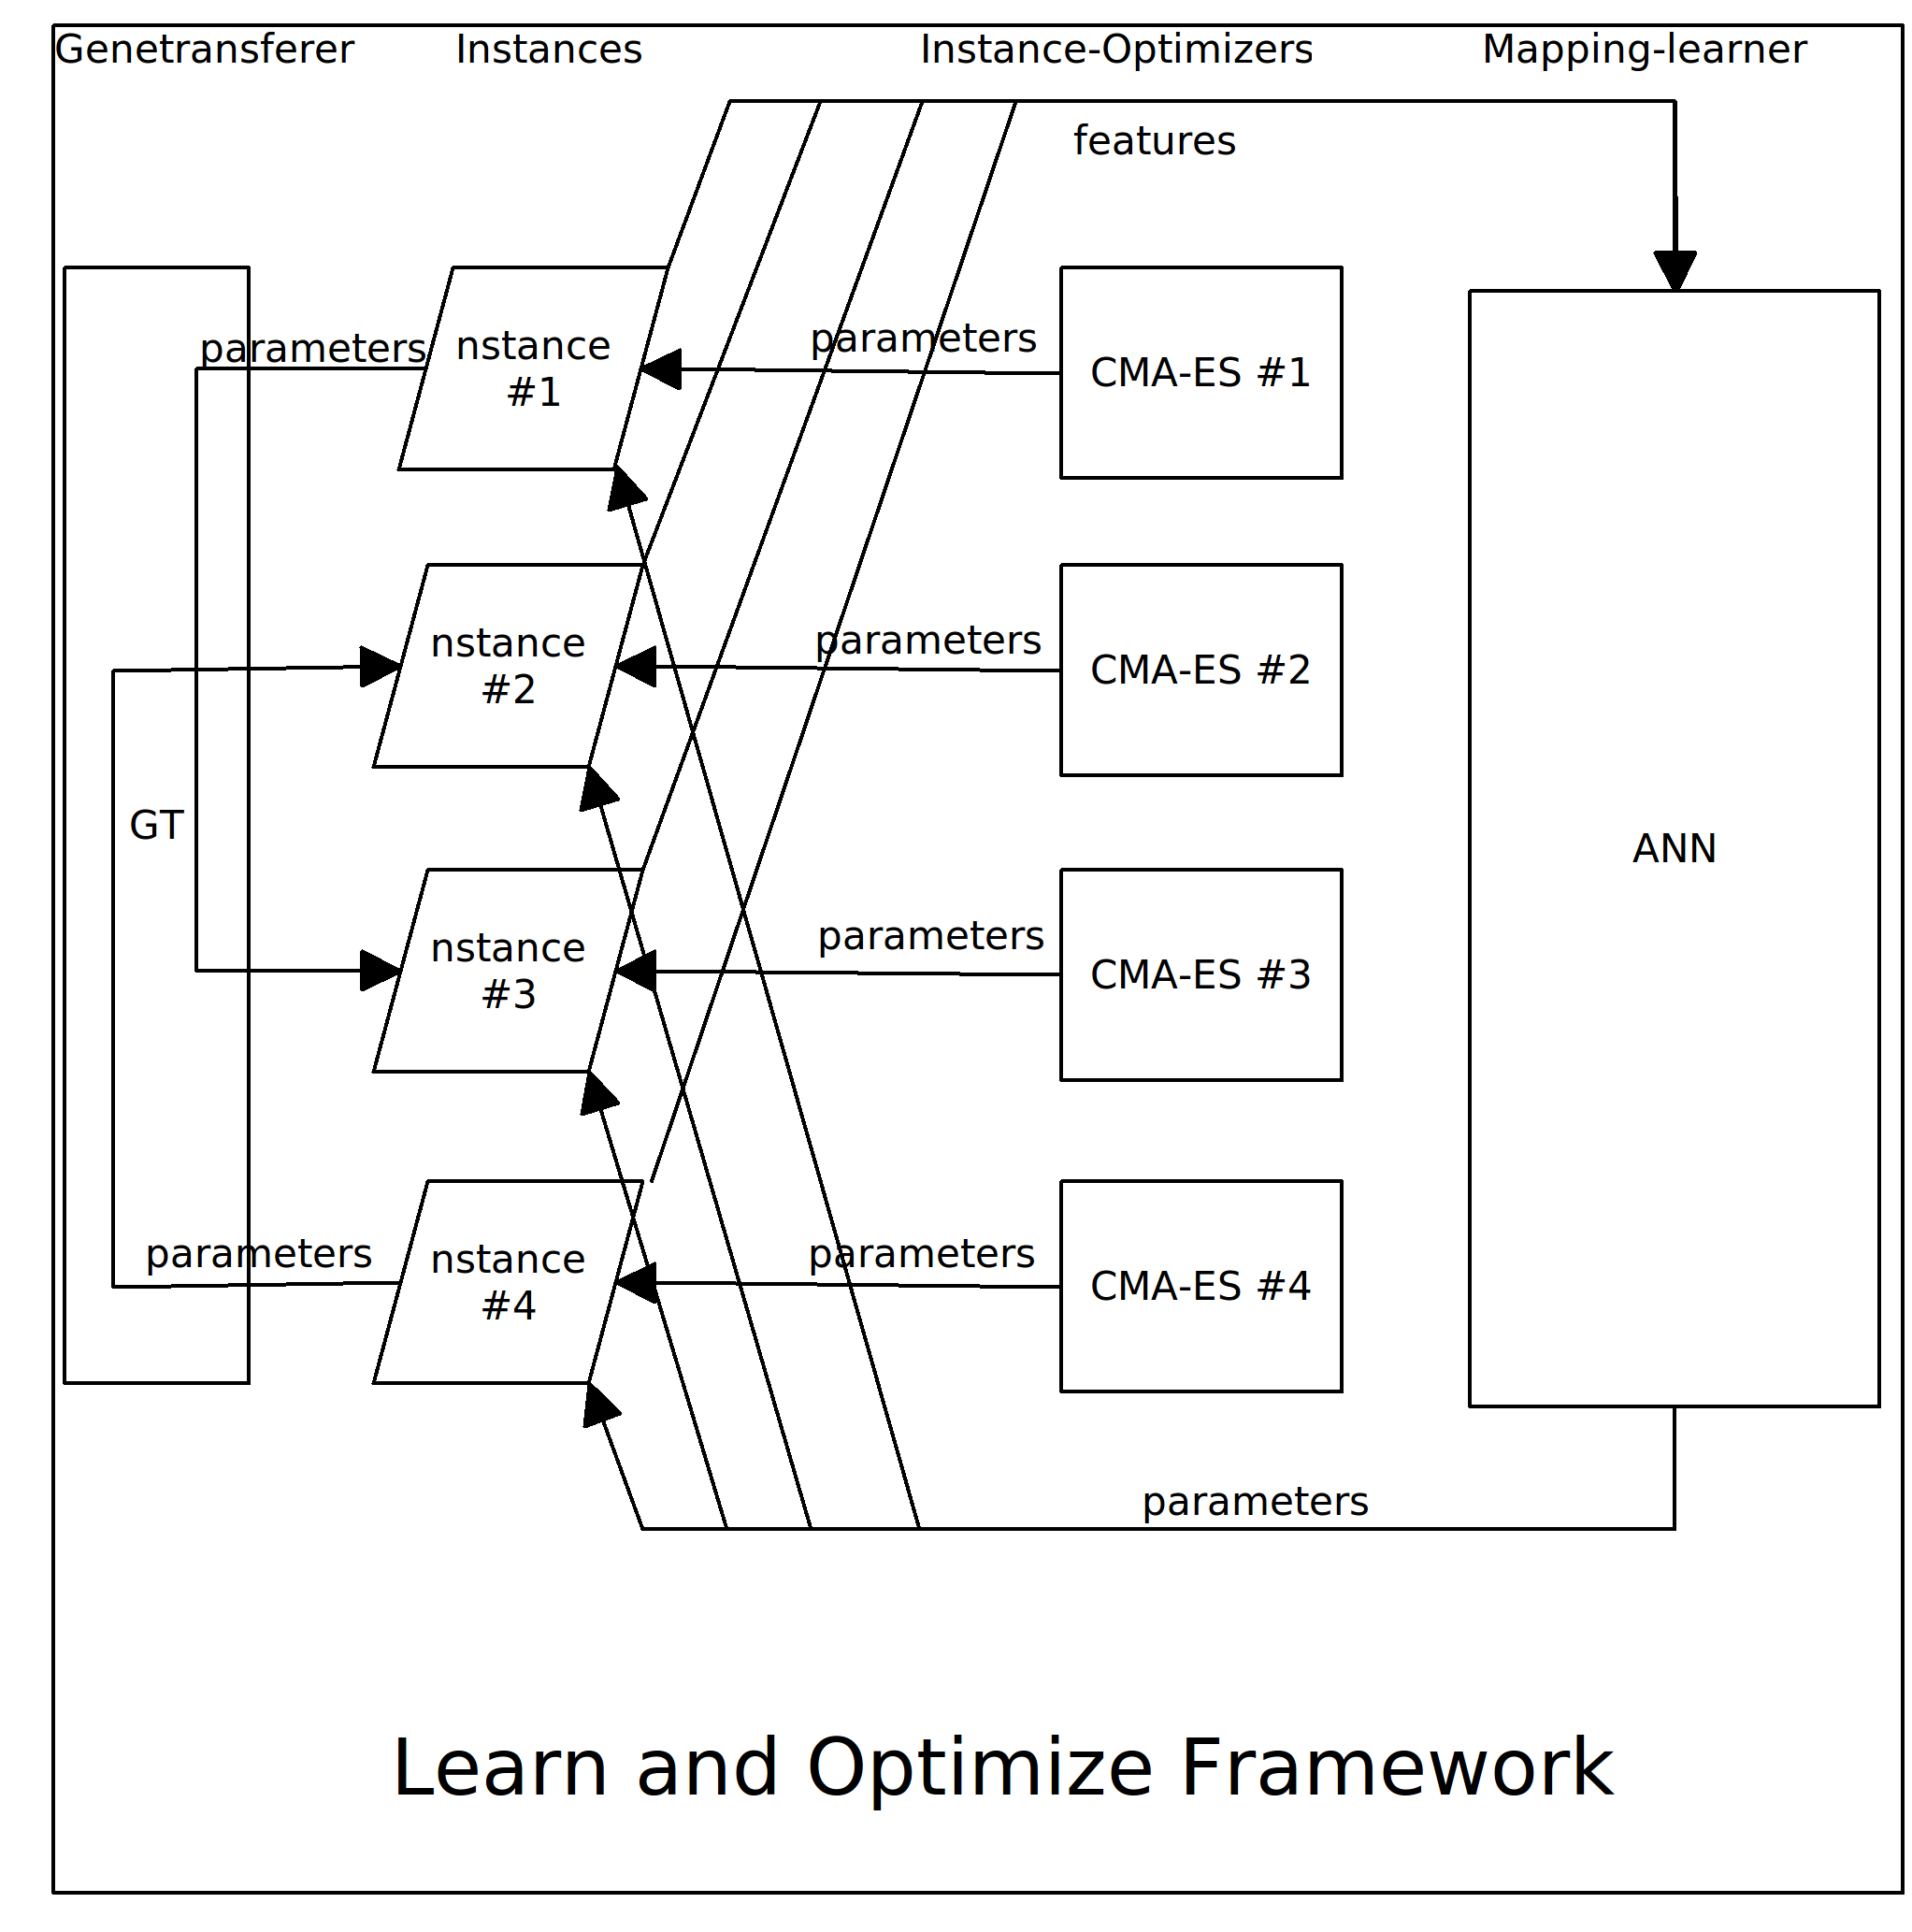
\includegraphics[width=0.5\textwidth]{lao.png}
  \caption{Flowchart of the Lao framework, displaying only 4 instances.}
\label{figure:laoflowchart}
\end{figure}



\begin{table*}[ht]
\centering
\begin{tabular}{l c c c c c c c}
\hline\hline
Domain & \# of & \# training & \# test &  ANN & quality-ratio & quality-ratio & quality-ratio \\ 
Name & iterations  & instances &  instances &  error & in LaO & ANN on train & ANN on test \\ 
\hline
Freecell& 16 & 108 & 230 & 0.1 & 1.09 & 1.05 & 1.04  \\
Grid & 10 & 55 & 124 & 0.09 & 1.09 & 1.05 & 1.03  \\
Mprime & 8 & 64 & 152 & 0.08 & 1.11 & 1.05 & 1.04   \\
\hline
\end{tabular}
\caption{Results by domains (only the actually usable training instances are shown). ANN-error is given as MSE, as returned by FANN. The quality-improvement ratio in Lao is that of the best parameter-set found by LaO.}
\label{table:domains}
\end{table*} 


\begin{table}[ht]
\centering
\begin{tabular}{l c c c}
\hline\hline
Name & Min & Max & Default \\ 
\hline
Probability of crossover & 0.0 & 1 & 0.8 \\
Probability of mutation & 0.0& 1& 0.2 \\
Rate of mutation add station& 0& 10& 1 \\
Rate of mutation delete station& 0& 10& 3 \\
Rate of mutation add atom& 0& 10& 1 \\
Rate of mutation delete atom& 0& 10& 1 \\
Mean average for mutations& 0.0& 1& 0.8 \\
Time interval radius& 0& 10& 2 \\
Maximum number of stations& 5& 50& 20 \\
Maximum number of nodes& 100& 100 000& 10 000 \\
Population size& 10& 300& 100 \\
Number of offspring & 100& 2 000& 700 \\
\hline
\end{tabular}
\caption{DaE parameters that are controlled by LaO}
\label{table:parameters}
\end{table} 

The implementation of LaO algorithm uses the Shark library \cite{shark08} for CMA-ES and the FANN library for ANN \cite{nissen}. To evaluate each parameter-setting with each instance,  a cluster was used, that has approximately 60 nodes, most of them with 4 cores, some with 8. However, this cluster is used by many researchers, therefore our algorithm was automatically scheduled to only use the spare CPU cycles on this cluster.

Moreover, since DaE is not deterministic, 11 independent runs were carried out for each DaE experiment with a given paramrter-set, and the fitness of this parameter set was taken to be the median fitness-value obtained by DaE.

\section{Results}
\label{section:results}

3 sample domains were selected from the Planning and Learning Part of IPC2011 (IPC): Freecell, Grid, and Mprime. For each of the domains, 100 instances were generated for training. Table \ref{table:domains} shows the data for each domain: from the 5 domain, only 3 had enough solvable instances to be used for the learning part. The Mean Square Error (MSE) of the trained ANN is shown for each domain. But because the fitness takes only few values, there can be multiple optimal parameter sets for the same instance, resulting in an unavoidable MSE. 
One iteration of LaO amounts to 5 iterations of CMA-ES, followed by one ANN training and one Genetransferer. Due to the time constraints, only 10 iterations of LaO were run on the Grid, hence CMA-ES was called 50 times in total.

The ANN had 3 fully connected layers, and the hidden layer had the same number of neurons than the input. In one iteration of LaO, the ANN was only trained for 50 iterations (aka epochs) 500 in total. After stopping LaO, retraining was made with 300 ANN epochs with the best data, because the ANN's saved directly from LaO may be under-trained. 

The controlled parameters of DaE are described in table \ref{table:parameters}. For a detailed description of these parameters, see \cite{BibGECCO:2010}. The feature-set consists of 12 features. The first 5 features are computed from the domain file, after the initial grounding of YAHSP: number of fluents, goals, predicates, objects and types. One further feature we think could even be more important is called mutex-density, which is the number of mutexes divided by the number of all fluent-pairs. We also kept 6 less important features: number of lines, words and byte-count - obtained by the linux command "wc" - of the instance and the domain file. These features were kept only for historical reasons: they were used in the beginning as some "dummy" features.

For evaluation the quality-improvement the quality-ratio metric defined in IPC competitions was used. A baseline experiments comes from the default parameter-setting. The ratio of the fitness value for the default parameter and the tuned parameter was computed and average was taken over the instances in the train or test-set. 

\begin{equation}Q=\frac{Fitness_{baseline}}{Fitness_{tuned}}\end{equation}

Table \ref{table:domains} presents several quality-improvement ratios. Label "in LaO" means that the best found parameter is compared to the default. Quality-improvement ratios for the retrained ANN on both the training-set and the test-set are also presented. As it can be seen on Table \ref{table:domains}, some quality-gain in training was consistently achieved, but the transfer of this improvement to the ANN-model was only partial. On the other hand, the ANN model generalizes excellently to the the independent test-set. Quality-improvement ratios dropped only by 0.01, i.e. the knowledge incorporated in the ANN was transferable to the test cases and usable almost to the same extent than for the train set.

\section{Conclusions and Future Work}
\label{section:conclusions}
\label{section:futurework}	

LaO was demonstrated to be capable of improving the quality of the DaE algorithm consistently, even though it was run only for a few iterations. On-going work is concerned with running LaO for an appropriate number of iterations. A clearly visible result is also that some of this quality-improvement can be incorporated into an ANN-model, which is also able to generalize excellently to an independent test-set.

Since LaO is only a framework, as indicated other kind of learning methods, and other kind of optimization techniques may be incorporated. If an ANN is used, the optimal structure has to be determined. Gene-transfer shall be improved so that chromosomes are transfered deterministically, measuring the similarity of instances by the similarity of their features.

Finally, the inter-domain generalization capability of LaO must be tested. However, the present results indicate that the current feature set is too small and should be extended for better results.


\section{Acknowledgements}
This work is funded through French ANR project DESCARWIN ANR-09-COSI-002.
% \section{Restrictions on Further Use}


\bibliographystyle{abbrv}
\bibliography{gecco2011brendelschoenauer}
\end{document}






